%%%%%%%%%%%%%%%%%%%%%%%%%%%%%%%%%%%%%%%%%%%%%%%%%%%%%%%%%%%%%%%%%%%%%%%%%%%%%%%%%%%%%%%%%%%
%                                    PhDthesis v0.1                                       %
%                            By Quan Zou <quan.zou@gmail.com>                             %
%                            Version 0.1 released 05/01/2014                              %
%%%%%%%%%%%%%%%%%%%%%%%%%%%%%%%%%%%%%%%%%%%%%%%%%%%%%%%%%%%%%%%%%%%%%%%%%%%%%%%%%%%%%%%%%%%
%
%
%------------------------------------------------------------------------------------------
% thesis chapter
%------------------------------------------------------------------------------------------
\chapter{Result}
\hskip 0.5in

\section{Rock result}

here is the result Figure~\ref{result:Rock}. 

  \begin{figure}[h!]
    \subfloat[\label{result:rock00}]{%
      %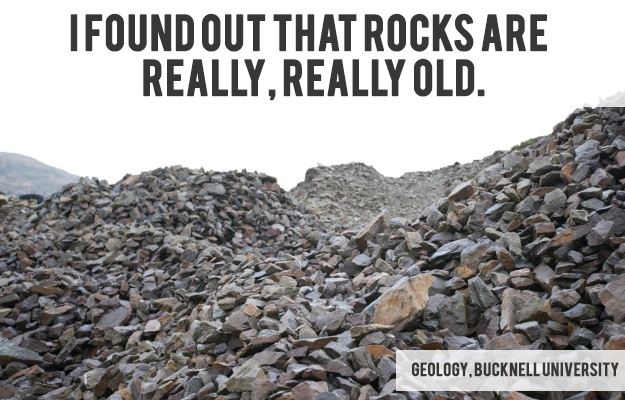
\includegraphics[natwidth=625bp,natheight=400bp, width=0.45\textwidth]{chap4/chap4figs/Rock.png}
      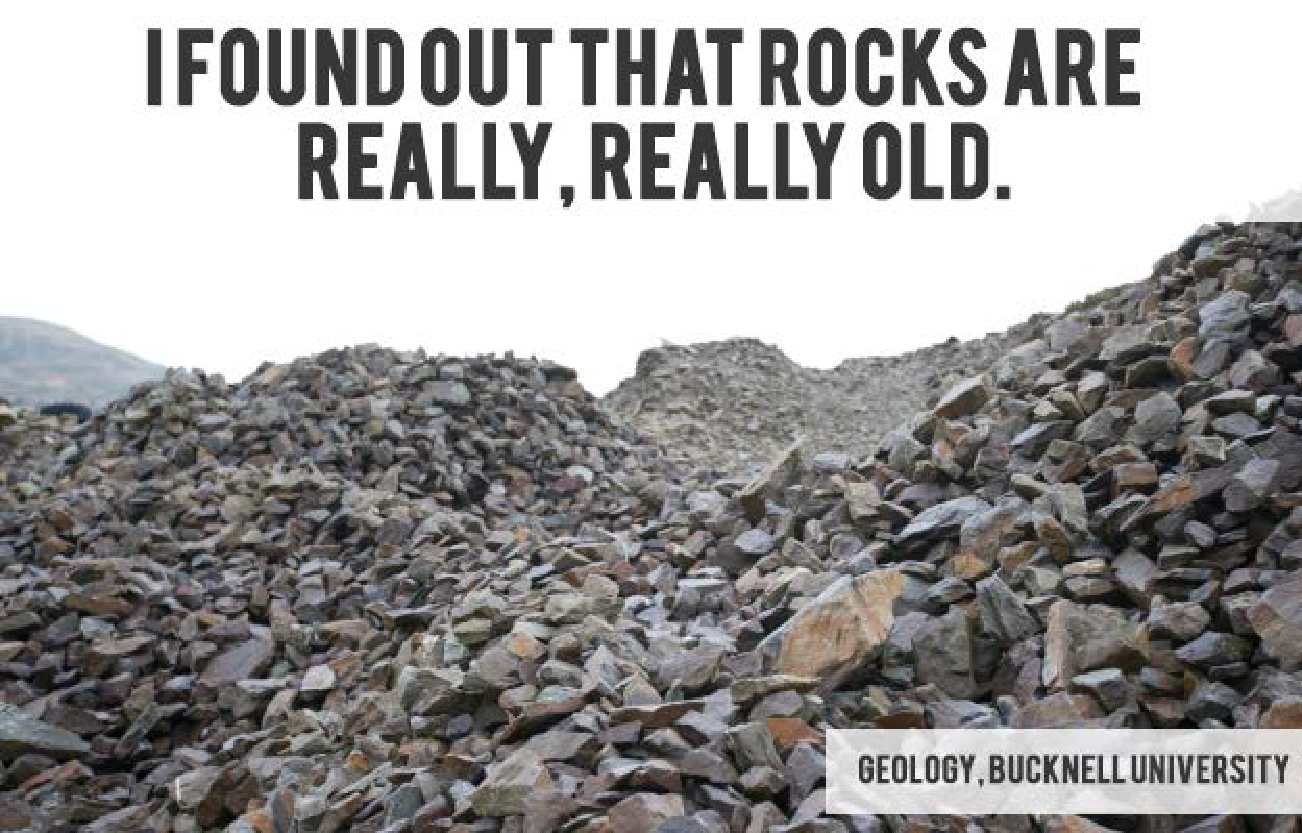
\includegraphics[bb=0 0 625 400, width=0.45\textwidth]{chap4/chap4figs/Rock.pdf}
    }
    \hfill
    \subfloat[\label{result:rock01}]{%
	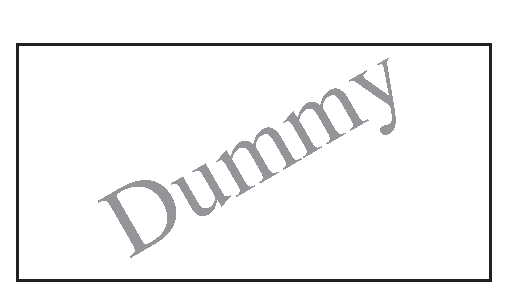
\includegraphics[bb=0 0 228 127, width=0.45\textwidth]{chap4/chap4figs/dummy.eps}
    }
    \caption{Rock photos}
		{(a) Rock and (b) eps dummy figure}
    \label{result:Rock}
  \end{figure} 
